\newcommand{\LLScan}[1]{

\begin{frame}{Likelihood scan for $C_{#1}$}
\includegraphics[width=\textwidth]{2020_04_28/figs/#1_Norm.png}
NB The straight line is a plotting artefact from \texttt{pyplot}
\end{frame}
}


\newcommand{\pull}[2]{
\begin{frame}{Pull distribution for #2 }
\includegraphics[width=\textwidth]{2020_04_28/figs/#1.png}
\end{frame}

}

\newcommand{\pullDist}[3]{
\begin{frame}{Pull distribution for $C_{#1}$ with the #3 tag}
\includegraphics[width=\textwidth]{2020_04_28/figs/pulls/#2_#1.png}
\end{frame}

}
\newcommand{\diffDist}[3]{
\begin{frame}{Pull distribution for $C_{#1}$ with the #3 tag}
\includegraphics[width=\textwidth]{2020_04_28/figs/diffs/#2_#1.png}
\end{frame}

}


\newcommand{\dists}[3]{
\begin{frame}{$C_{#1}$ with the #3}
\begin{columns}
\begin{column}{0.5\textwidth}
\includegraphics[width=\textwidth]{2020_04_28/figs/diffs/#2_#1.png}
\end{column}
\begin{column}{0.5\textwidth}
\includegraphics[width=\textwidth]{2020_04_28/figs/pulls/#2_#1.png}
\end{column}
\end{columns}

Left : Distribution of $C_{#1}^\text{Fit} - C_{#1}^\text{True}$,

right : $(C_{#1}^\text{Fit} - C_{#1}^\text{True})/\sigma C_{#1}^\text{Fit}$
\end{frame}

}

\newcommand{\alldists}[2]{
\dists{00}{#1}{#2}
\dists{01}{#1}{#2}
\dists{10}{#1}{#2}
\dists{02}{#1}{#2}
\dists{11}{#1}{#2}
\dists{02}{#1}{#2}
}

\begin{frame}{Overview}
    \begin{itemize}
        \item After considering physical constraints on $\dd$, we change our proposed ``CP-polynomial'' to an ``anti-symmetric'' polynomial
        \item Widen the range for the likelihood scan for each component
        \item Perform a pull study for the ``anti-symmetric'' polynomial
    \end{itemize}
\end{frame}
\begin{frame}
    Given that 
    \begin{equation}
        \dd(\MM,\MP) = -\dd(\MP,\MM),
    \end{equation}
    and that the model $\dd$ ($\dd^\text{model}$) satisfies this, any correction to $\dd^\text{model}$ ($f(\MM,\MP)$) must also satisfy (1), i.e. the so-called ``CP-Negative'' polynomial, which we will rename to the anti-symmetric polynomial since the function is anti-symmetric along the line $\MM=\MP$, using the parameterisation $w_\pm = (z_+ \pm z_-)/2$ where $z_\pm$ is a re-scaled $m^2_\pm$ such that $z_\pm \in (-1,1)$,
    \begin{equation}
        f(w_-,w_+) = \sum_{i=0}^{N_\text{Order}} \sum_{j=0}^{N_\text{Order} - i} C_{ij} P_{i}(w_+) P_{2j+1}(w_-)
    \end{equation}
\end{frame}

\begin{frame}{$\dd$ plot}
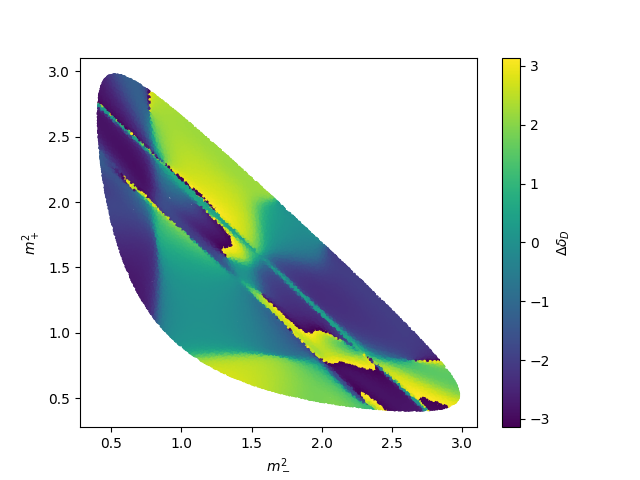
\includegraphics[width=\textwidth]{2020_04_28/figs/dd.png}
\end{frame}
\LLScan{00}
\LLScan{01}
\LLScan{10}
\LLScan{02}
\LLScan{11}
\LLScan{20}

\begin{frame}{Pull Studies}
\begin{enumerate}
    \item Generate $N=10000$ sample from the Belle-BaBar 2018 model
    \item Tags are \KK, \Kspiz, \Kppim, \Kmpip, \Kspipi and the combined tag
    \item \Kppim and \Kmpip tags are modified such that the wrong sign couplings are $-0.0537\pm0.032i$ (back of envelope calculation)
    \item Fit with $N_\text{Order}=2$ polynomial
\end{enumerate}{}
\end{frame}

\pull{KK}{\KK}
\pull{Kmpip}{\Kmpip}
\pull{Kppim}{\Kppim}
\pull{Kspi0}{\Kspiz}
\pull{Kspipi}{\Kspipi}
\pull{Comb}{Combined tags}

